% Overleaf: upload the whole ZIP and select proposal.tex as Main document.
% The source Word document is unchanged. Control passages and the system
% figure are updated to position PI in the FPGA, with no current controller.
\documentclass[11pt,letterpaper]{article}
\usepackage[T1]{fontenc}
\usepackage[utf8]{inputenc}
\usepackage{lmodern}
\usepackage[margin=0.8in]{geometry}
\usepackage{amsmath,amssymb,booktabs,tabularx,array,microtype}
\usepackage{graphicx,pdflscape,float,enumitem}
\usepackage[hidelinks]{hyperref}
\setlength{\parindent}{0pt}
\setlength{\parskip}{6pt}
\setlength{\emergencystretch}{2em}
\widowpenalty=10000
\clubpenalty=10000
\setlist{nosep,leftmargin=*}
\newcommand{\checkitem}{\item[$\square$]}
\title{Magnetic Levitation Project Proposal}
\author{Stephen Kanti Mahanty and Ben Lertwachara\\ENGR 155}
\date{}
\begin{document}
\maketitle
\vspace{-1.4em}

\section{Project overview}
Our project will suspend a permanent magnet carrying an object below an
electromagnet. The magnet, carrier, and object will total 10 g. The webpage
will command motion between 10 and 20 mm surface gaps. Two Hall sensors,
mounted above and below the electromagnet, will measure magnetic field.
We will combine both readings with measured coil current to estimate the
target's height. A position PI controller will adjust PWM duty to hold the
requested gap; there will be no current-feedback controller.

We will use the STM32L432KC MCU, UPduino FPGA, and course ESP8266 Wi-Fi
module. Gap \(d\) is the distance from the bottom of the coil to the top of
the suspended magnet. We will demonstrate the round trips and position
tolerance listed in the specifications and check gap with a ruler. The
webpage will display requested gap, estimated gap, current, and faults on a
real-time graph, include a stop button, and allow updates to the position
PI constants.

\section{MCU and FPGA design}
The MCU will read the MCP3204 ADC over SPI using three separate channels:
Hall sensor A, Hall sensor B, and coil current. A timer will start scans at
5 kHz, with DMA moving SPI data. At 1 kHz, the MCU will estimate gap from
the calibrated sensor readings and measured current. USART1 will connect
to the ESP8266 at 125000 baud. The MCU will handle the web interface,
telemetry, and transfer of requested gap and PI constants.

The MCU will send estimated gap, requested gap, measured current, and status
to the FPGA over SPI. The FPGA will execute the position PI controller at
1 kHz using DSP blocks and generate 20 kHz PWM. Its output is duty directly;
there is no requested-current signal or current PI loop. Current measurement
supports magnetic-field compensation, telemetry, and protection. The FPGA
will turn off drive after 50 ms without valid commands. A MOSFET, gate
driver, and flyback diode will switch the 12 V coil; a shunt and amplifier
will measure current. An E-stop and overcurrent comparator will disable
the driver directly. The MCU will also provide a drive-permit signal.

SPI DMA is our new MCU peripheral use; the DSP position controller is our
new FPGA logic; the ADC and magnetic sensing circuit are our new external
hardware. SPI links carry commands and replies. Logic uses 3.3 V and shares
ground with the coil circuit. Figure~\ref{fig:architecture} shows the
updated architecture. PI gain changes will be range-checked and applied
together at a control-update boundary. Drive limits and integrator
anti-windup will be implemented and tested.

\begin{landscape}
\begin{figure}[p]
 \centering
 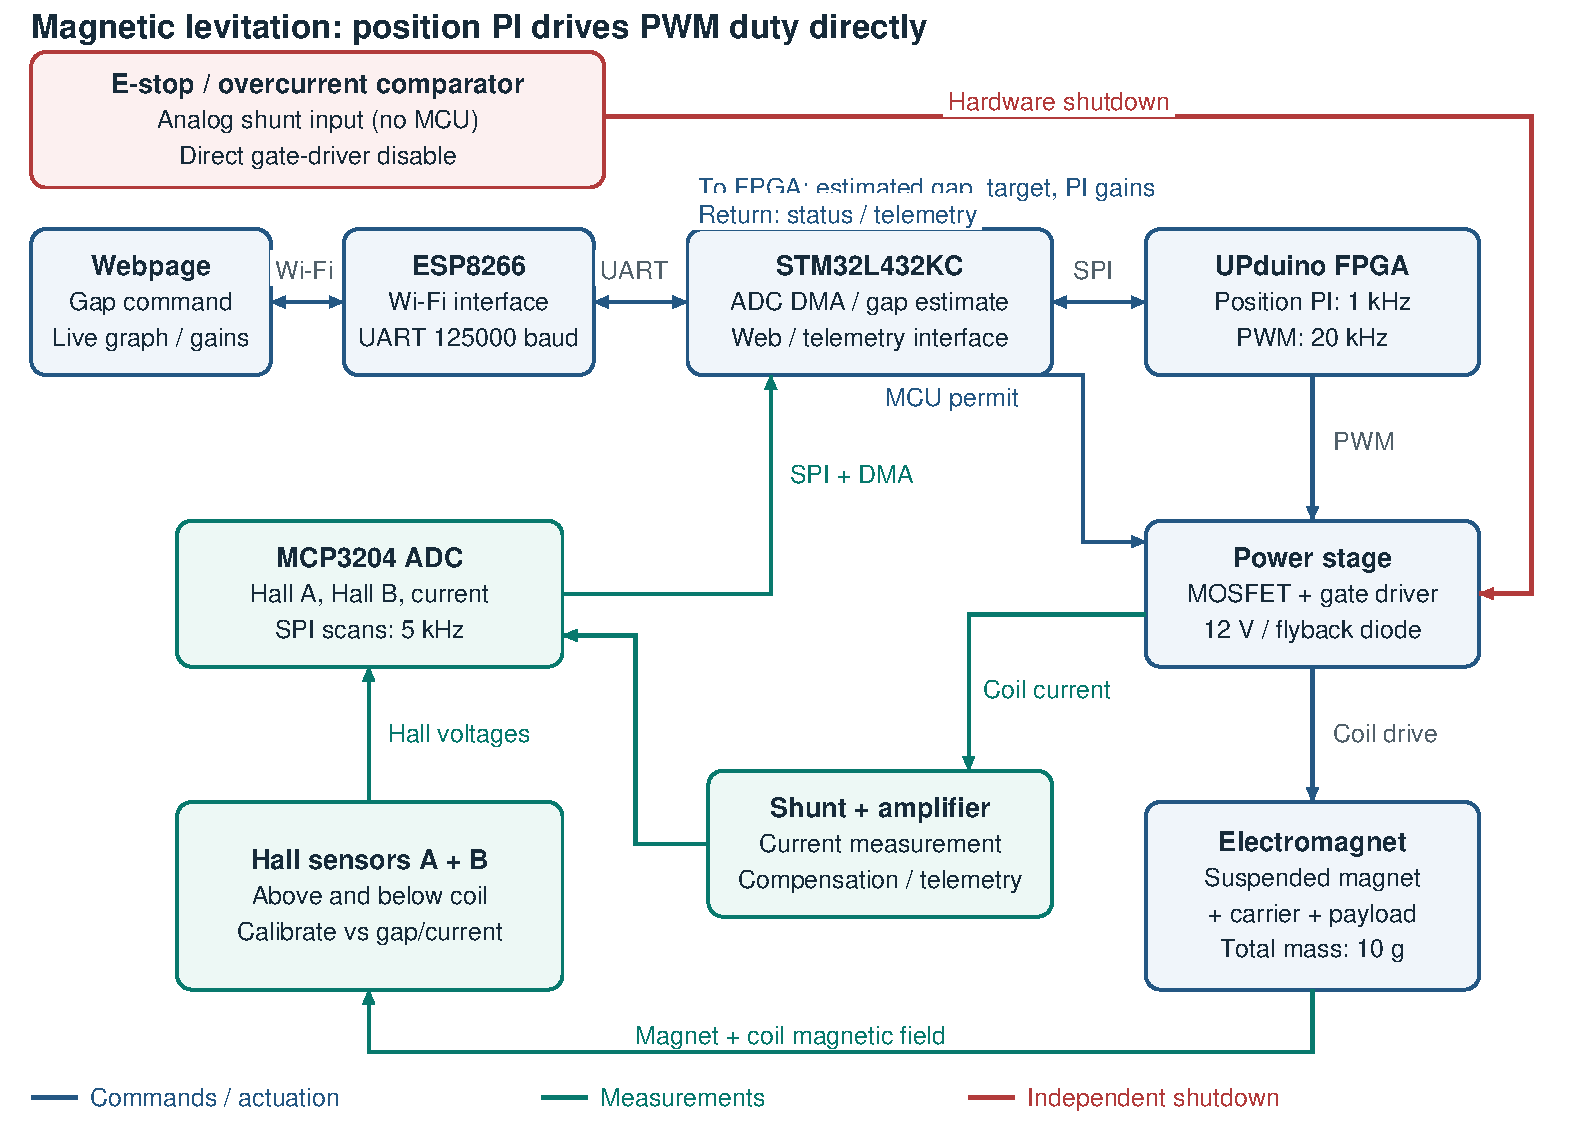
\includegraphics[width=0.95\linewidth]{assets/system_architecture.pdf}
 \caption{FPGA position PI drives PWM duty. The MCU handles ADC/DMA, gap
 estimation, and the web interface. The analog overcurrent comparator
 disables drive independently of the MCU. There is no current controller.}
 \label{fig:architecture}
\end{figure}
\end{landscape}

\section{Biggest challenge}
Our biggest challenge is separating the target's field from the coil's
field. We will mount Hall sensors A and B above and below the electromagnet
and calibrate both readings at known gaps and coil currents on a plastic
fixture. The MCU will read the sensors on separate ADC channels, combine
their readings in software, and compensate for the coil field using
measured current. We will verify the estimated gap against ruler
measurements over the 10--20 mm operating range. The ADC's limited
differential mode cannot directly subtract both full Hall outputs. A catch
tray and upper stop will protect against falls and the target snapping upward.

\section{Current needed to lift an object at 12 V}
Voltage alone does not tell us how much weight we can lift. We need the
total mass \(m\) of the magnet, carrier, and object, plus the coil geometry
and magnet strength. For a first estimate, assume a small aligned permanent
magnet below a thin air-core coil. Let \(N\) be the number of turns, \(a\)
the mean coil radius, \(\mu\) the magnet's dipole moment, and \(z\) the
distance from the coil plane to the magnet's center. Use meters and
kilograms in the equations.
\begin{align}
 B(z)&=\frac{\mu_0NIa^2}{2(a^2+z^2)^{3/2}},\\
 F&\simeq\mu\left|\frac{\mathrm dB}{\mathrm dz}\right|=K(z)I,\\
 K(z)&=\frac{3\mu_0N\mu a^2z}{2(a^2+z^2)^{5/2}},\qquad
 I_{\mathrm{hold}}(z)=\frac{mg}{K(z)}.
\end{align}
Here \(\mu_0=4\pi\times10^{-7}\,\mathrm{H/m}\) and
\(g=9.81\,\mathrm{m/s^2}\). To move up by \(\Delta h\) mm from
\(z_0\), the final distance is \(z_1=z_0-\Delta h/1000\). Current must
provide enough force throughout the move, not just at the endpoint. To
accelerate upward at \(a_{\mathrm{up}}\), use
\(I=m(g+a_{\mathrm{up}})/K(z)\). Center distance \(z\) differs from
surface gap \(d\); we will convert between them using the actual dimensions.

\subsection{Example for a 10 g magnet and payload}
For a sizing calculation, use \(N=500\), \(a=10\,\mathrm{mm}\),
\(\mu=0.050\,\mathrm{A\,m^2}\), and \(R=8\,\Omega\). These are
calculation assumptions, not selected parts. The table covers center
distances of 10--20 mm; actual center distances include the coil and magnet
offsets from surface gap \(d\). With ideal PWM,
\(D\simeq IR/12\) and coil heating is \(P=I^2R\).
\begin{center}
\begin{tabular}{rrrr}
\toprule
Center distance \(z\) & Holding current & 12 V duty & Coil heating\\
\midrule
20 mm & 5.819 A & 388\% & 270.9 W\\
15 mm & 2.643 A & 176\% & 55.9 W\\
10 mm & 1.178 A & 79\% & 11.1 W\\
\bottomrule
\end{tabular}
\end{center}
For this example, \(12/8=1.50\,\mathrm A\) is the ideal full-on current
limit. Holding at \(z=20\,\mathrm{mm}\) requires 5.819 A, so this example
coil cannot deliver the required range at 12 V. A 10 mm upward move from
\(z=20\) to 10 mm requires the largest holding current at the start. For
a one-second move with equal acceleration and deceleration,
\(a_{\mathrm{up}}=4(0.010)/1^2=0.040\,\mathrm{m/s^2}\); the initial
current becomes 5.842 A. A duty above 100\% means the supply cannot provide
the required current.

We will select the final coil and magnet using measured force versus gap
and current. The assembly must support the 10 g target over the full
10--20 mm surface-gap range at 12 V. We will measure hot resistance,
inductance, and temperature and check that the supply covers
\(IR+L\,\mathrm dI/\mathrm dt\) and circuit losses. An iron core and finite
magnet dimensions change the simple air-core estimate. Stable suspension
will be verified by the demonstration specifications.

\section{Timing and measurement calculations}
At 1 MHz SPI, a 24-clock ADC reading takes \(24\,\mu\mathrm s\).
Including a \(1\,\mu\mathrm s\) gap, current plus two Hall readings takes
\(75\,\mu\mathrm s\). An 8-byte FPGA exchange takes about
\(68\,\mu\mathrm s\) with chip-select gaps. Together this uses
\(143\,\mu\mathrm s\) of a \(200\,\mu\mathrm s\) scan period, leaving
\(57\,\mu\mathrm s\) for setup and processing. We will check the actual
timing with a logic analyzer. The FPGA's position PI update is 1 kHz;
ADC acquisition and SPI exchanges may run at the faster 5 kHz scan rate.

The 12-bit ADC has 4096 levels:
\(3.3\,\mathrm V/4096=0.806\,\mathrm{mV}\) per count. With a
\(0.100\,\Omega\) shunt and gain of 20, current resolution is about
\(0.403\,\mathrm{mA}\) per count. At 1.18 A the shunt dissipates 0.139 W.
A 24 MHz FPGA clock divided by 1200 gives 20 kHz PWM.

\section{Stability calculation: nominal 10 mm operating point}
The controller is position PI driving duty directly, with no current
controller. For a real 10 mm surface gap \(d_0\), the force model must use
\(z_0=d_0+\Delta_g\), where \(\Delta_g\) accounts for coil-plane and
magnet-center offsets. The numerical illustration below uses
\(z_0=10\,\mathrm{mm}\) in the thin-coil/point-magnet approximation;
it is not a validated result for a finite assembly at 10 mm surface gap.

For \(m=0.010\,\mathrm{kg}\), the equilibrium force is
\(F_0=mg=0.0981\,\mathrm N\). Using the sizing model above gives
\begin{equation}
 k_f=K(z_0)=0.0833041\,\mathrm{N/A},\qquad
 i_0=\frac{mg}{k_f}=1.17761\,\mathrm A,\qquad u_0=\frac{Ri_0}{12}=0.78508.
\end{equation}
Define \(x=d-d_0\), \(j=i-i_0\), and upward force
\(F\simeq mg-k_xx+k_fj\). The local destabilizing force slope is
\begin{equation}
 k_x=-\left.\frac{\partial F}{\partial d}\right|_0
 =mg\left(\frac{5z_0}{a^2+z_0^2}-\frac1{z_0}\right)
 =14.715\,\mathrm{N/m}.
\end{equation}
With downward displacement positive, the mechanical equation, position PI,
and electrical equation are
\begin{align}
 m\ddot x+c\dot x-k_xx+k_fj&=0,\\
 \delta u=K_px+K_i\eta,\qquad\dot\eta&=x,\\
 L\dot j+Rj-k_f\dot x&=V_s\delta u.
\end{align}
Here \(c\) is passive mechanical damping, \(L\) is differential coil
inductance, \(\delta u=u-u_0\), and \(V_s=12\,\mathrm V\).
The PI gains have units \(\mathrm{m^{-1}}\) and
\(\mathrm{m^{-1}s^{-1}}\), respectively. The induced-voltage term follows
reciprocal magnetic coupling; it is not a current controller.

Taking Laplace transforms and eliminating current gives the characteristic
equation
\begin{equation}
\boxed{\begin{aligned}
0={}&mLs^4+(mR+cL)s^3+(cR-k_xL+k_f^2)s^2\\
   &+(k_fV_sK_p-k_xR)s+k_fV_sK_i.
\end{aligned}}
\end{equation}
For the explicitly assumed \(L=10\,\mathrm{mH}\) and negligible passive
damping \(c=0\), this becomes
\begin{equation}
\boxed{\begin{aligned}
0={}&0.0001s^4+0.08s^3-0.140210s^2\\
   &+(0.999649K_p-117.72)s+0.999649K_i.
\end{aligned}}
\end{equation}
The negative \(s^2\) coefficient violates a necessary Routh--Hurwitz
condition. Therefore this assumed continuous-time plant cannot be
stabilized by position PI tuning alone. For illustration,
\(K_p=150\,\mathrm{m^{-1}}\), \(K_i=100\,\mathrm{m^{-1}s^{-1}}\)
produce poles
\begin{equation}
 s=-802.247,\quad -2.9963,\quad 2.6214\pm j\,20.2237\ \mathrm{s^{-1}},
\end{equation}
so an oscillatory mode grows. These are unstable example gains, not
recommended settings. A necessary damping/electrical condition is
\begin{equation}
 cR+k_f^2>k_xL,
\end{equation}
which requires \(L<0.4716\,\mathrm{mH}\) if \(c=0\), or
\(c>0.01753\,\mathrm{N\,s/m}\) if \(L=10\,\mathrm{mH}\).
Passing this condition alone does not guarantee stability.

For completeness, if the quartic coefficients are \(A_4,\ldots,A_0\),
all must be positive, with \(A_3A_2>A_4A_1\) and
\(A_3A_2A_1>A_4A_1^2+A_3^2A_0\). We will measure the final coil's
force slopes, resistance, inductance, and damping at the actual surface
gap before selecting gains. The 1 kHz sampled controller, held PWM duty,
sensor filtering, and delays must then be checked for poles inside the
unit circle. The companion \texttt{calculation\_summary.tex} provides the
derivation and sampled-state formulation. The 10 mm distance improves
static lifting feasibility; it does not establish stable suspension.

\section{Position resolution and stability verification}
Position resolution will be determined from the calibrated relationship
between the two Hall readings, measured current, and gap. ADC voltage
resolution alone is not a position-resolution specification. We will
measure estimator noise and bias at fixed known gaps, then report the
smallest reliably distinguishable position change.

We will evaluate stability separately by recording requested and estimated
gap during holds, commanded moves, and repeatable disturbances. Position
band and recovery time will be stated separately. The ruler-based
demonstration band below is \(\pm5\,\mathrm{mm}\); finer claims require
correspondingly accurate position measurements. The calculation above
identifies a design condition to resolve before stable suspension can be
claimed.

\clearpage
\section{Project specifications}
These are proposed demonstration targets. We will use one magnet, carrier,
and object totaling 10 g. Professors can check each box during the
demonstration using a ruler, stopwatch, webpage, and scope or logic analyzer.
Excellence includes all proficiency checks.

\subsection{Hardware and levitation}
\textbf{Proficiency}
\begin{itemize}
 \checkitem Use the webpage to move from 20 to 10 mm and back five times
 without contact.
\end{itemize}
\textbf{Excellence}
\begin{itemize}
 \checkitem Complete five 20-to-10 mm round trips, reaching within
 \(\pm5\,\mathrm{mm}\) of each requested gap.
\end{itemize}

\subsection{Control and webpage}
\textbf{Proficiency}
\begin{itemize}
 \checkitem Show requested gap, estimated gap, coil current, and fault state
 on a real-time webpage graph, with no visible latency between the object
 and graph during the demonstration.
 \checkitem Allow updates to the position PI constants from the webpage.
\end{itemize}
\textbf{Excellence}
\begin{itemize}
 \checkitem Demonstrate visibly noticeable movement of the magnet through
 webpage control across the controllable range.
\end{itemize}

\section{Bill of materials and budget}
\begin{tabularx}{\linewidth}{@{}X r@{}}
\toprule
Parts & Planned cost\\
\midrule
NUCLEO-L432KC, UPduino, ESP8266; bench supply and frame & Course kit / stockroom*\\
2 DRV5055 Hall sensors; MCP3204 ADC; INA240A1 amplifier & \$16\\
0.100 \(\Omega\), 1 W shunt; UCC27511 driver; MOSFET; flyback diode & \$6\\
Coil, magnet and carrier; adapters, resistors and capacitors & \$14\\
Fuse and connectors*; shipping and tax allowance & \$3 + \$10\\
\midrule
\textbf{Estimated total} & \textbf{\$49}\\
\bottomrule
\end{tabularx}

*Stockroom availability is unconfirmed. Costs are allowances; final coil
and power-switch parts depend on testing.

\section{Schedule and division of work}
\begin{tabularx}{\linewidth}{@{}l X X@{}}
\toprule
Week & Stephen & Ben\\
\midrule
1--2 & Measure coil force; build driver and FPGA PWM &
Read ADC; calibrate Hall and current readings\\
3--4 & Implement and tune FPGA position PI after plant characterization;
build frame and stops & Validate gap estimate; verify loop timing and
position measurements\\
5--6 & Webpage, shutdown tests, and schematic &
Motion tests, checkoff measurements, and report\\
\bottomrule
\end{tabularx}

\section*{Calculation references}
\begin{enumerate}
\raggedright
\item OpenStax, \emph{University Physics, Volume 2},
\href{https://openstax.org/books/university-physics-volume-2/pages/12-4-magnetic-field-of-a-current-loop}{Sec.~12.4: Magnetic Field of a Current Loop}.
\item H.~H. Woodson and J.~R. Melcher, \emph{Electromechanical Dynamics},
Part I, Chs.~3 and 5. MIT OpenCourseWare.
\href{https://ocw.mit.edu/courses/res-6-003-electromechanical-dynamics-spring-2009/pages/part-i/}{Online textbook and chapters}.
\item University of Illinois, ECE 486 Handbook, Lecture 7, Routh--Hurwitz criterion.
\href{https://courses.physics.illinois.edu/ece486/sp2026/documentation/handbook/lec07.html}{Online lecture notes}.
\item A.~V. Oppenheim, A.~S. Willsky, with S.~H. Nawab,
\emph{Signals and Systems}, 2nd ed., Chs.~9--11.
\href{https://ocw.mit.edu/courses/6-003-signals-and-systems-fall-2011/pages/readings/}{MIT reading guide}.
\end{enumerate}
\end{document}
